\chapter{कोशिकाओं और विषाणुओं के जीनोम}\label{ch:b1:genomes}

दो मीटर \omterm{def:b1:nucleic-acids:chain}{DNA} छह माइक्रोमीटर आरपार के किसी केंद्रक में मुड़ा हुआ है, और इस
तरह मुड़ा है कि बीस हज़ार \omterm{def:b1:genomes:gene}{जीनों} में से कोई भी मिनटों में ढूँढ़ा और पढ़ा
जा सके। कोई जीवाणु डेढ़ मिलीमीटर उस \omterm{def:b1:cell-unit-of-life:cell}{कोशिका} में मोड़ लेता है जो एक हज़ार
गुना छोटी है, और उसे हर बीस मिनट में नक़ल कर लेता है। कोई \omterm{def:b1:genomes:virus}{विषाणु} किसी
\omterm{def:b1:proteins:peptide}{प्रोटीन} खोल में कुछ हज़ार अक्षर ढोता है और उन्हें उस \omterm{def:b1:cell-unit-of-life:cell}{कोशिका} से पढ़वाता है
जो उसकी अपनी नहीं। यह अध्याय \emph{\omterm{def:b1:genomes:genome}{जीनोम}} का ---
यानी किसी \omterm{def:b1:organism-environment:organism}{जीव} के पूरे \omterm{def:b1:nucleic-acids:chain}{DNA} का --- एक भौतिक वस्तु के रूप में वर्णन करता है:
जीवाणुओं का, \omterm{def:b1:cell-unit-of-life:prokeuk}{सुकेंद्रकी} \omterm{def:b1:cell-unit-of-life:cell}{कोशिकाओं} का, \omterm{def:b1:cell-unit-of-life:prokeuk}{कोशिकांगों} का और \omterm{def:b1:genomes:virus}{विषाणुओं} का \omterm{def:b1:nucleic-acids:chain}{DNA}
कैसे संगठित है, उसमें \omterm{def:b1:genomes:gene}{जीनों} के अलावा क्या है, और उसकी मात्रा उस \omterm{def:b1:organism-environment:organism}{जीव} के
बारे में इतना कम क्यों बताती है जो उसे ढोता है।

\section{जीवाणु जीनोम}

\begin{definition}[जीनोम, गुणसूत्र, केंद्रकाभ]\label{def:b1:genomes:genome}
किसी \omterm{def:b1:cell-unit-of-life:cell}{कोशिका} का \emph{जीनोम}\index{जीनोम} उसके सारे \omterm{def:b1:nucleic-acids:chain}{DNA} का जोड़ है:
यानी हर उस \omterm{def:b1:proteins:peptide}{प्रोटीन} तथा \omterm{def:b1:nucleic-acids:chain}{RNA} की जानकारी जो वह बना सकती है, और वे
अनुक्रम जो नियंत्रित करते हैं कि वे कब बनें। \emph{गुणसूत्र}\index{गुणसूत्र}
एक \omterm{def:b1:nucleic-acids:chain}{DNA} अणु है, उन \omterm{def:b1:proteins:peptide}{प्रोटीनों} सहित जो उसे सजाते हैं। किसी जीवाणु में
प्रायः एक होता है, वर्तुल, दस से चालीस लाख \omterm{thm:b1:nucleic-acids:helix}{क्षारक युग्मों} का
(\emph{E. coli}: $\num{4.6e6}$, \qty{1.5}{mm} लंबा), जो \omterm{def:b1:cell-unit-of-life:cell}{कोशिकाद्रव्य} के
किसी क्षेत्र में मुड़ा रहता है, यानी \emph{केंद्रकाभ}\index{केंद्रकाभ}
में, और जिसके चारों ओर कोई झिल्ली नहीं होती। गुणसूत्र के अलावा अनेक
जीवाणु \emph{प्लास्मिड}\index{प्लास्मिड} ढोते हैं: यानी कुछ हज़ार से कुछ
लाख युग्मों के छोटे वृत्त, एक से लेकर सैकड़ों प्रतियों में, जो अपने आप
प्रतिकृत होते हैं और वैकल्पिक \omterm{def:b1:genomes:gene}{जीन} ढोते हैं --- प्रतिजैविक प्रतिरोध,
विषाक्त पदार्थ, और स्वयं को किसी दूसरी \omterm{def:b1:cell-unit-of-life:cell}{कोशिका} में भेजने की मशीनरी।
\end{definition}

\begin{proposition}[कोई जीवाणु अपना गुणसूत्र कैसे मोड़ता है]\label{prop:b1:genomes:supercoiling}
\index{अतिकुंडलन}
जिस वर्तुल \omterm{def:b1:nucleic-acids:chain}{DNA} के सिरे घूम न सकें उसे किसी रबड़ बैंड की तरह ऐंठा जा सकता
है: \emph{अतिकुंडलन}। \emph{टोपोआइसोमरेज़} कहलाते \omterm{def:b1:enzymes:enzyme}{एंजाइम} लड़ियों को
काटते, पार कराते और फिर जोड़ देते हैं ताकि फेरे जुड़ें या हटें; और
\emph{गाइरेज़} \omterm{def:b1:water-small-molecules:atp}{ATP} से ऋणात्मक अतिकुंडलियाँ डालता है, जो कुंडली को कम कस
देती हैं और उसे एक ही साथ अधिक संहत तथा खोलने में आसान बनाती हैं।
\emph{E. coli} का \omterm{def:b1:genomes:genome}{गुणसूत्र} कोई पचास फंदों में सजा है, और हर फंदा
स्वतंत्र रूप से अतिकुंडलित तथा किसी \omterm{def:b1:proteins:peptide}{प्रोटीन} अंतर्भाग से बँधा है, इसलिए वे
\qty{1.5}{mm} लगभग एक माइक्रोमीटर के \omterm{def:b1:genomes:genome}{केंद्रकाभ} में समा जाते हैं --- यानी
एक हज़ार गुना संहतीकरण --- और फिर भी बाक़ी को छेड़े बिना कोई भी फंदा पढ़ने
या नक़ल करने के लिए खोला जा सकता है। छोटे क्षारीय \omterm{def:b1:proteins:peptide}{प्रोटीन}
(\omterm{def:b1:genomes:nucleosome}{हिस्टोन} जैसे, यद्यपि \omterm{def:b1:genomes:nucleosome}{हिस्टोनों} से असंबंधित) पूरे \omterm{def:b1:nucleic-acids:chain}{DNA} को जगह-जगह मोड़ते
और जोड़ते हैं।
\end{proposition}

\begin{omfigure}
\begin{tikzpicture}[font=\footnotesize, line cap=round]
  % relaxed circle
  \draw[very thick, omDef] (0,0) circle (1.1);
  \node[anchor=north, align=center] at (0,-1.35) {शिथिल वृत्त\\ (प्रति फेरा 10.5 bp)};
  % supercoiled: figure-eight / plectoneme
  \draw[very thick, omDef, domain=0:360, samples=240, smooth, variable=\t] plot ({4.3+1.05*cos(\t)}, {0.32*sin(4*\t)});
  \node[anchor=north, align=center] at (4.3,-1.35) {ऋणात्मक रूप से अतिकुंडलित:\\ कम कसा, संहत};
  \draw[->, thick] (1.35,0.15) -- (3.1,0.15) node[midway, above, align=center] {गाइरेज़ (ATP)};
  \draw[->, thick] (3.1,-0.25) -- (1.35,-0.25) node[midway, below, align=center] {टोपोआइसोमरेज़ I};
  % looped nucleoid
  \fill[omProp!40] (8.7,0) circle (0.35);
  \foreach \a in {0,45,...,315} {
    \draw[very thick, omDef] (8.7,0) .. controls ({8.7+1.6*cos(\a-20)},{1.6*sin(\a-20)}) and ({8.7+1.6*cos(\a+20)},{1.6*sin(\a+20)}) .. (8.7,0);
  }
  \node[anchor=north, align=center] at (8.7,-1.35) {केंद्रकाभ: किसी प्रोटीन अंतर्भाग पर\\ लगभग पचास अतिकुंडलित फंदे};
\end{tikzpicture}

{\small कोई वर्तुल \omterm{def:b1:genomes:genome}{गुणसूत्र} शिथिल, अतिकुंडलित, और फंदों में सजा हुआ।
अतिकुंडलन अणु को संहत करता है और वह ऊर्जा संचित करता है जो उसे खोलने में
मदद देती है; और फंदे एक बार में एक ही क्षेत्र खुलने देते हैं।}
\end{omfigure}

\begin{example}[एक सघन जीनोम]\label{ex:b1:genomes:dense}
\emph{E. coli} के \omterm{def:b1:genomes:genome}{गुणसूत्र} की \qty{4.6}{Mb} में से \qty{88}{\%}
\omterm{def:b1:proteins:peptide}{प्रोटीन} के लिए कूट है: यानी लगभग \num{1000} युग्मों के कोई \num{4300}
\omterm{def:b1:genomes:gene}{जीन}, जो सिर से पूँछ जमे हैं और जिनके बीच सौ युग्म हैं, और जिनमें से अनेक
\emph{ऑपेरॉनों} में समूहबद्ध होकर साथ अनुलेखित होते हैं (\cref{ch:b1:expression-control})।
\qty{5}{kb} का कोई \omterm{def:b1:genomes:genome}{प्लास्मिड} तीन \omterm{def:b1:genomes:gene}{जीन} ढो सकता है और पचास
प्रतियों में हो सकता है; और वह जो प्रतिरोध \omterm{def:b1:genomes:gene}{जीन} ढोता है वह किसी अस्पताल के
वार्ड के जीवाणुओं में हफ़्तों में संयुग्मन से फैल सकता है, यानी किसी भी
उत्परिवर्तन के उठ सकने से तेज़।
\end{example}

\section{सुकेंद्रकी जीनोम: क्रोमैटिन}

\begin{definition}[न्यूक्लियोसोम, क्रोमैटिन]\label{def:b1:genomes:nucleosome}
\index{न्यूक्लियोसोम}\index{हिस्टोन}\index{क्रोमैटिन}
किसी \omterm{def:b1:cell-unit-of-life:prokeuk}{सुकेंद्रकी} केंद्रक में \omterm{def:b1:nucleic-acids:chain}{DNA} \omterm{def:b1:proteins:peptide}{प्रोटीनों} पर लिपटा रहता है: \qty{147}{}
\omterm{thm:b1:nucleic-acids:helix}{क्षारक युग्म} आठ \emph{हिस्टोनों} के किसी अष्टक के चारों ओर 1.7 फेरे लेते
हैं (H2A, H2B, H3, H4 में से हर एक के दो, जो लाइसीन तथा
आर्जिनीन से समृद्ध छोटे \omterm{def:b1:proteins:peptide}{प्रोटीन} हैं और फ़ॉस्फ़ेटों को उदासीन करते हैं),
और इस तरह \qty{11}{nm} आरपार का एक
\emph{न्यूक्लियोसोम}\index{न्यूक्लियोसोम} बनता है; न्यूक्लियोसोम
हर \qty{200}{} युग्मों के आसपास एक-दूसरे के पीछे आते हैं, किसी डोरी पर
मनकों की तरह, और एक पाँचवाँ हिस्टोन, H1, हर मनके को सील कर देता है। यह
\emph{क्रोमैटिन} और आगे मुड़ता है: \qty{30}{nm} के किसी तंतु में, दसियों
हज़ार युग्मों के उन फंदों में जो किसी \omterm{def:b1:proteins:peptide}{प्रोटीन} ढाँचे पर बँधे हैं,
और --- विभाजन के समय --- मध्यावस्था \omterm{def:b1:genomes:genome}{गुणसूत्र} की संहत छड़ों में, जो नंगे
\omterm{def:b1:nucleic-acids:chain}{DNA} से दस हज़ार गुना छोटी हैं।
\emph{सुक्रोमैटिन} अंतरावस्था का वह ढीला, जीन-समृद्ध, अनुलेखित रूप है;
और \emph{विषमक्रोमैटिन} वह संघनित, जीन-दरिद्र रूप जो संहत ही रहता है
(\omterm{def:b1:genomes:karyotype}{सेंट्रोमियरों} के चारों ओर, सिरों पर, और किसी बंद कर दिए गए
X \omterm{def:b1:genomes:genome}{गुणसूत्र} पर)।
\end{definition}

\begin{omfigure}
\begin{tikzpicture}[font=\footnotesize, >=Stealth, line cap=round]
  % level 1: double helix line
  \draw[very thick, omDef] (0,5.4) -- (3.2,5.4);
  \node[anchor=west, align=left] at (3.5,5.4) {द्विकुंडली, \qty{2}{nm}};
  % level 2: beads on a string
  \draw[thick, omDef] (0,4.2) -- (3.2,4.2);
  \foreach \x in {0.4,1.2,2.0,2.8} { \fill[omProp!70] (\x,4.2) circle (0.22); \draw[thick, omDef] (\x,4.2) circle (0.3); }
  \node[anchor=west, align=left] at (3.5,4.2) {न्यूक्लियोसोम, \qty{11}{nm}: किसी हिस्टोन अष्टक के चारों ओर \qty{147}{bp},\\ हर \qty{200}{bp} पर --- संहतीकरण $\times 6$};
  % level 3: 30 nm fibre (zigzag stack)
  \foreach \i in {0,...,9} { \fill[omProp!70] (0.2+0.3*\i,{3.0+0.18*(-1)^\i}) circle (0.17); }
  \node[anchor=west, align=left] at (3.5,3.0) {\qty{30}{nm} तंतु: चिने हुए न्यूक्लियोसोम --- $\times 40$};
  % level 4: loops on scaffold
  \draw[very thick, gray] (0,1.5) -- (3.2,1.5);
  \foreach \x in {0.4,1.2,2.0,2.8} { \draw[thick, omProp!80!black] (\x,1.5) .. controls (\x-0.35,2.3) and (\x+0.35,2.3) .. (\x,1.5); }
  \node[anchor=west, align=left] at (3.5,1.8) {किसी ढाँचे पर \qtyrange{50}{100}{kb} के फंदे, \qty{300}{nm} --- $\times 1000$};
  % level 5: metaphase chromosome
  \draw[very thick, omThm, fill=omThm!30, rounded corners=4pt] (0.9,-0.3) rectangle (1.4,1.0);
  \draw[very thick, omThm, fill=omThm!30, rounded corners=4pt] (1.7,-0.3) rectangle (2.2,1.0);
  \fill[omThm!60!black] (1.55,0.45) ellipse (0.45 and 0.13);
  \node[anchor=west, align=left] at (3.5,0.35) {मध्यावस्था गुणसूत्र, \qty{1400}{nm} आरपार: $\times \num{10000}$\\ (\qty{10}{\micro m} में \qty{8.5}{cm} DNA)};
\end{tikzpicture}

{\small \omterm{def:b1:cell-unit-of-life:prokeuk}{सुकेंद्रकी} \omterm{def:b1:nucleic-acids:chain}{DNA} के जमाव के स्तर, कुंडली से लेकर मध्यावस्था
\omterm{def:b1:genomes:genome}{गुणसूत्र} तक। हर स्तर संहतीकरण को गुणा करता है; और पूरा जोड़ दस हज़ार तक
पहुँचता है।}
\end{omfigure}

\begin{omfigure}
\begin{minipage}[b]{0.46\linewidth}\centering
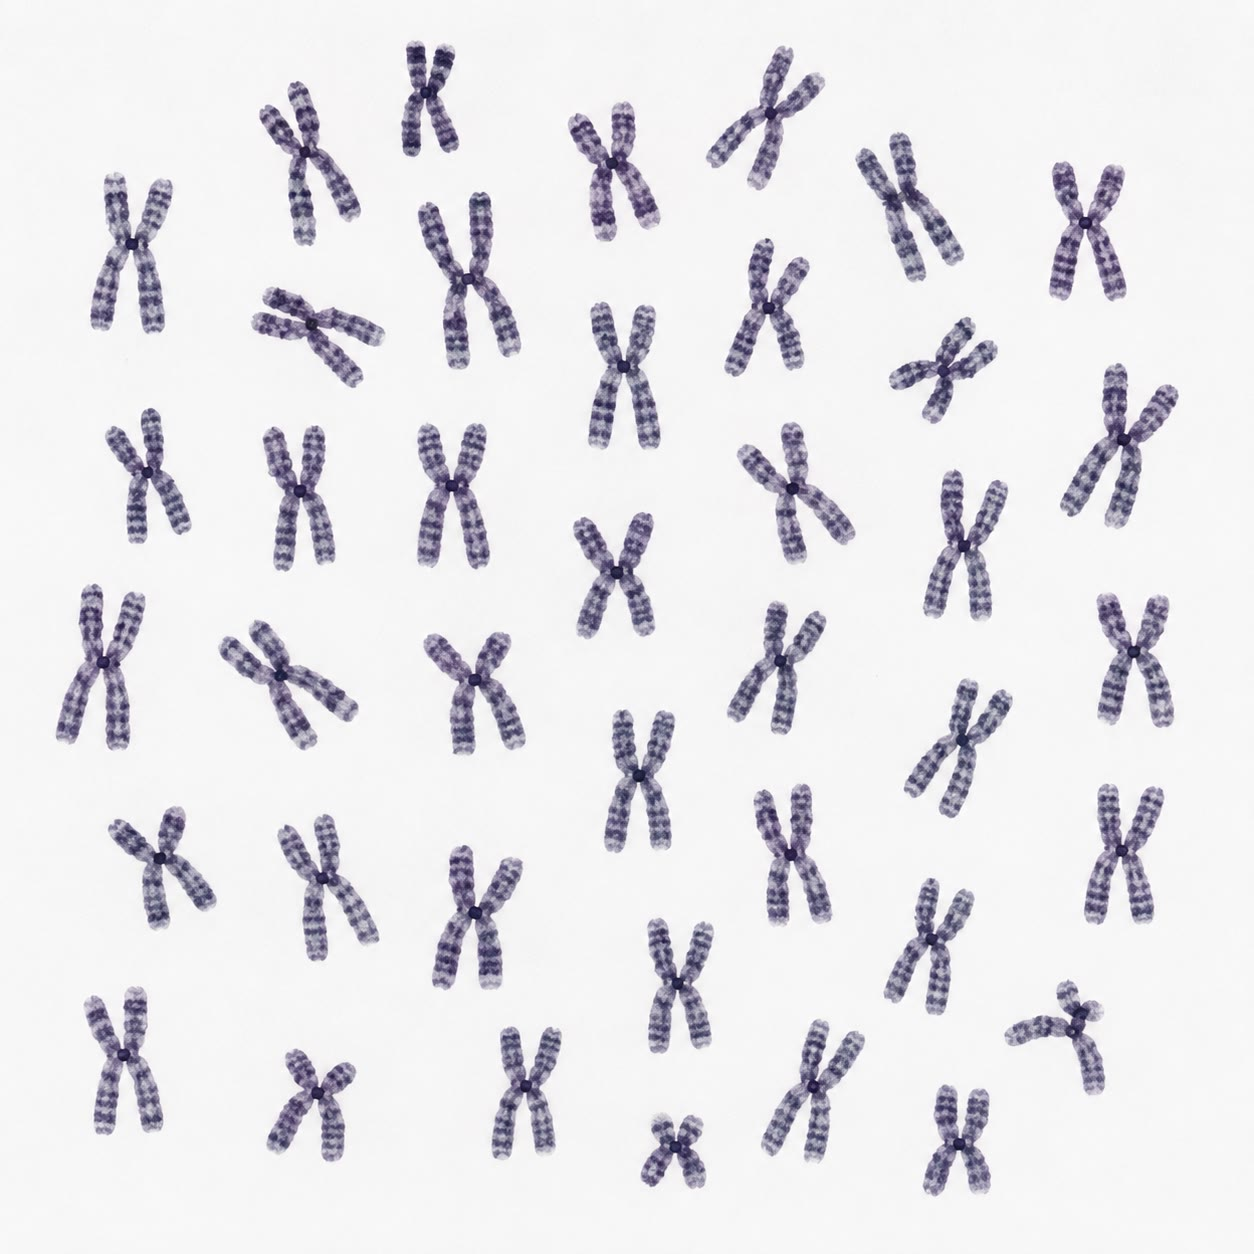
\includegraphics[width=0.94\linewidth]{images/book3/ai/b3-17-metaphase-spread.jpg}
\end{minipage}\hfill
\begin{minipage}[b]{0.5\linewidth}\centering
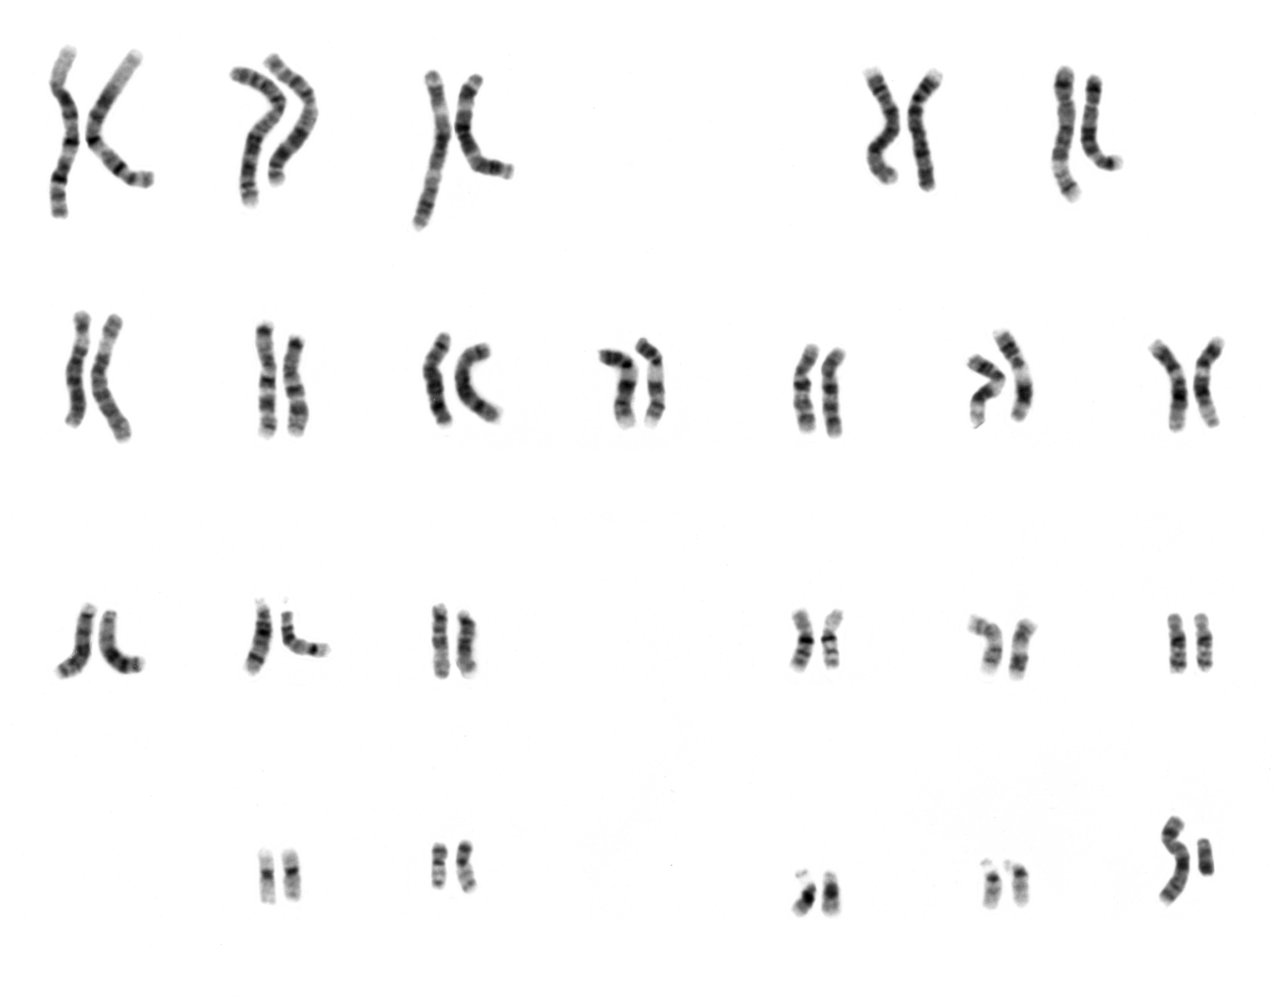
\includegraphics[width=0.96\linewidth]{images/book3/karyotype.png}
\end{minipage}

{\small बाएँ: एक मानव \omterm{def:b1:cell-unit-of-life:cell}{कोशिका} के \omterm{def:b1:genomes:genome}{गुणसूत्र}, जो मध्यावस्था पर रोकी गई किसी
\omterm{def:b1:cell-unit-of-life:cell}{कोशिका} से फैलाए गए हैं। दाएँ: वही \omterm{def:b1:genomes:genome}{गुणसूत्र} आकार और पट्टियों के अनुसार
किसी \omterm{def:b1:genomes:karyotype}{गुणसूत्र-चित्र} में छाँटे हुए --- बाईस जोड़े और XY, कुल छियालीस।
\omterm{def:b1:genomes:karyotype}{गुणसूत्र-चित्र}: राष्ट्रीय मानव \omterm{def:b1:genomes:genome}{जीनोम} अनुसंधान संस्थान, सार्वजनिक
अधिकार-मुक्त।}
\end{omfigure}

\begin{definition}[गुणसूत्र-चित्र, सेंट्रोमियर, टीलोमियर]\label{def:b1:genomes:karyotype}
\index{गुणसूत्र-चित्र}\index{सेंट्रोमियर}\index{टीलोमियर}
\emph{गुणसूत्र-चित्र} किसी \omterm{def:b1:cell-unit-of-life:cell}{कोशिका} के \omterm{def:b1:genomes:genome}{गुणसूत्रों} का वह समुच्चय है जो
आकार और पट्टी-प्रतिरूप से छाँटा गया हो: मनुष्यों में 23 जोड़े हैं (22
अलिंगसूत्र और XY या XX), कुल $\num{6.4e9}$ \omterm{thm:b1:nucleic-acids:helix}{क्षारक युग्म}, यानी \qty{2.2}{m};
सबसे बड़ा \omterm{def:b1:genomes:genome}{गुणसूत्र} \qty{250}{Mb} रखता है, सबसे छोटा \qty{50}{}। हर रैखिक
\omterm{def:b1:genomes:genome}{गुणसूत्र} एक \emph{सेंट्रोमियर} ढोता है, यानी वह सिकुड़ा हुआ क्षेत्र जहाँ
प्रतिकृतिकरण के बाद दोनों प्रतियाँ जुड़ी रहती हैं और जहाँ तर्कु जुड़ता है
(\cref{ch:b1:replication-mitosis}), और दो \emph{टीलोमियर}, यानी सिरों पर
के वे दोहराए गए अनुक्रम जो उन्हें टूटा हुआ \omterm{def:b1:nucleic-acids:chain}{DNA} समझे जाने से और हर
प्रतिकृतिकरण पर छोटा होने से बचाते हैं।
\end{definition}

\begin{proposition}[जीनोम का आकार जटिलता नहीं मापता]\label{prop:b1:genomes:cvalue}
\index{C-मान विरोधाभास}
\begin{center}
\small
\begin{tabular}{lrr}
\hline
\omterm{def:b1:organism-environment:organism}{जीव} & \omterm{def:b1:genomes:genome}{जीनोम} (Mb) & प्रोटीन-कूटलेखी \omterm{def:b1:genomes:gene}{जीन} \\
\hline
\emph{E. coli} & 4.6 & \num{4300} \\
खमीर & 12 & \num{6000} \\
फल-मक्खी & 140 & \num{14000} \\
मनुष्य & 3200 & \num{20000} \\
मक्का & 2300 & \num{40000} \\
फेफड़ा-मछली & \num{130000} & $\approx\num{20000}$ \\
\emph{Paris japonica} (एक कुमुदिनी) & \num{150000} & $\approx\num{30000}$ \\
\hline
\end{tabular}
\end{center}
\omterm{def:b1:cell-unit-of-life:prokeuk}{सुकेंद्रकियों} में \omterm{def:b1:genomes:genome}{जीनोम} का आकार एक हज़ार गुना तक बदलता है, और उसका \omterm{def:b1:genomes:gene}{जीनों}
की संख्या या \omterm{def:b1:organism-environment:organism}{जीव} की जटिलता से कोई संबंध नहीं (यही
\emph{\omterm{prop:b1:genomes:cvalue}{C-मान विरोधाभास}} है): कोई फेफड़ा-मछली मनुष्य से चालीस गुना \omterm{def:b1:nucleic-acids:chain}{DNA}
ढोती है और \omterm{def:b1:genomes:gene}{जीन} उससे अधिक नहीं। फ़र्क़ \omterm{def:b1:genomes:gene}{जीनों} का नहीं, उनके बीच के \omterm{def:b1:nucleic-acids:chain}{DNA} का
है।
\end{proposition}

\section{किसी जीनोम में क्या होता है}

\begin{definition}[किसी जीन की शारीरिकी]\label{def:b1:genomes:gene}
\index{जीन}\index{एक्सॉन}\index{इंट्रॉन}\index{उन्नायक}
\emph{जीन} \omterm{def:b1:nucleic-acids:chain}{DNA} का वह खंड है जो किसी क्रियाशील \omterm{def:b1:nucleic-acids:chain}{RNA} में अनुलेखित होता है
--- प्रायः किसी एक \omterm{def:b1:proteins:peptide}{प्रोटीन} के संदेशवाहक में। किसी \omterm{def:b1:cell-unit-of-life:prokeuk}{सुकेंद्रकी}
प्रोटीन-कूटलेखी जीन में होते हैं: एक \emph{उन्नायक}, यानी ऊपर-प्रवाह का
वह अनुक्रम जहाँ अनुलेखन शुरू होता है और नियंत्रित होता है; \emph{एक्सॉन},
यानी वे भाग जो परिपक्व संदेश में रखे जाते हैं; \emph{इंट्रॉन}, यानी वे
भाग जो अनुलेखित होकर काट दिए जाते हैं (\cref{ch:b1:gene-expression});
संदेश के दोनों सिरों पर के अनूदित न होने वाले क्षेत्र; और एक समापक। किसी
मानव जीन का औसत \qty{27}{kb} है जिसमें आठ एक्सॉन मिलकर
\qty{1.5}{kb} बनाते हैं: यानी किसी प्रारूपिक जीन का उन्नीस-बीसवाँ भाग
इंट्रॉन है। जीवाणु जीनों में इंट्रॉन नहीं होते।
\end{definition}

\begin{omfigure}
\begin{tikzpicture}[font=\footnotesize, >=Stealth, line cap=round]
  \draw[very thick, gray] (0,0) -- (12.6,0);
  \fill[omExo!50] (0.2,-0.18) rectangle (1.6,0.18); \node[anchor=north] at (0.9,-0.25) {उन्नायक};
  \fill[omDef!70] (1.6,-0.25) rectangle (2.4,0.25);
  \fill[omDef!70] (4.6,-0.25) rectangle (5.6,0.25);
  \fill[omDef!70] (8.4,-0.25) rectangle (9.0,0.25);
  \fill[omDef!70] (10.9,-0.25) rectangle (12.0,0.25);
  \node[anchor=south, omDef!70!black] at (2.0,0.3) {एक्सॉन 1};
  \node[anchor=south, omDef!70!black] at (5.1,0.3) {एक्सॉन 2};
  \node[anchor=south, omDef!70!black] at (8.7,0.3) {एक्सॉन 3};
  \node[anchor=south, omDef!70!black] at (11.45,0.3) {एक्सॉन 4};
  \node[anchor=north] at (3.5,-0.3) {इंट्रॉन 1};
  \node[anchor=north] at (7.0,-0.3) {इंट्रॉन 2};
  \node[anchor=north] at (9.95,-0.3) {इंट्रॉन 3};
  \draw[->, thick, omExo!70!black] (1.6,0.75) -- (2.6,0.75); \node[anchor=south, font=\scriptsize] at (2.6,0.85) {अनुलेखन यहाँ शुरू होता है};
  \node[anchor=north, align=center, gray] at (6.3,-0.9) {कोई प्रारूपिक मानव जीन: \qty{27}{kb}, जिसमें \qty{1.5}{kb} एक्सॉन;\\ परिपक्व संदेशवाहक में एक्सॉन जोड़ दिए जाते हैं, इंट्रॉन फेंक दिए जाते हैं};
\end{tikzpicture}

{\small एक \omterm{def:b1:cell-unit-of-life:prokeuk}{सुकेंद्रकी} \omterm{def:b1:genomes:gene}{जीन}: एक \omterm{def:b1:genomes:gene}{उन्नायक}, और \omterm{def:b1:genomes:gene}{एक्सॉन} (रखे गए) जो \omterm{def:b1:genomes:gene}{इंट्रॉनों}
(अनुलेखन के बाद हटाए गए) से एकांतर में हैं। दबे हुए पैमाने पर बनाया गया
--- असली \omterm{def:b1:genomes:gene}{जीन} में \omterm{def:b1:genomes:gene}{इंट्रॉन} \omterm{def:b1:genomes:gene}{एक्सॉनों} से बीस गुना लंबे होते।}
\end{omfigure}

\begin{proposition}[मानव जीनोम की जनगणना]\label{prop:b1:genomes:census}
\index{स्थानांतरणीय तत्व}\index{पुनरावृत्त DNA}
\qty{3.2}{Gb} में से: लगभग \qty{1.5}{\%} \omterm{def:b1:proteins:peptide}{प्रोटीन} के लिए कूट है; \qty{25}{\%}
\omterm{def:b1:genomes:gene}{इंट्रॉन} है; \qty{45}{\%} \emph{स्थानांतरणीय तत्वों} के अवशेष हैं
--- यानी उन अनुक्रमों के जो स्वयं को नई जगहों पर नक़ल कर लेते हैं और
अधिकतर कब के मर चुके हैं (अकेला Alu तत्व, \qty{300}{bp} का, दस लाख
प्रतियों में मौजूद है, यानी \omterm{def:b1:genomes:genome}{जीनोम} का दसवाँ भाग); \qty{8}{\%} क्रम में
लगी छोटी पुनरावृत्तियाँ हैं (उपग्रह \omterm{def:b1:nucleic-acids:chain}{DNA}, \omterm{def:b1:genomes:karyotype}{सेंट्रोमियरों} तथा टीलोमियरों
पर); और बाक़ी वह अद्वितीय अकूटलेखी अनुक्रम है जिसमें वे \omterm{def:b1:genomes:gene}{उन्नायक}, संवर्धक
और \omterm{def:b1:nucleic-acids:chain}{RNA} \omterm{def:b1:genomes:gene}{जीन} आते हैं जो अभिव्यक्ति नियंत्रित करते हैं। अनेक \omterm{def:b1:genomes:gene}{जीन} उन
\emph{कुलों} के हैं जो द्विगुणन से उठे (ग्लोबिन, घ्राण ग्राही ---
जिनमें से एक हज़ार हैं), और \omterm{def:b1:genomes:genome}{जीनोम} हज़ारों \emph{छद्मजीन} रखता है, यानी
मरी हुई प्रतियाँ जो अब काम नहीं करतीं। \omterm{def:b1:genomes:genome}{जीनोम} कोई अभिकल्पना नहीं, एक
अभिलेख है।
\end{proposition}

\begin{omfigure}
\begin{tikzpicture}[font=\footnotesize]
  \def\R{2.1}
  % slices: coding 1.5, introns 25, transposons 45, satellite 8, other 20.5
  \fill[omThm!70] (0,0) -- (90:\R) arc (90:84.6:\R) -- cycle;
  \fill[omDef!50] (0,0) -- (84.6:\R) arc (84.6:-5.4:\R) -- cycle;
  \fill[omProp!50] (0,0) -- (-5.4:\R) arc (-5.4:-167.4:\R) -- cycle;
  \fill[omExo!50] (0,0) -- (-167.4:\R) arc (-167.4:-196.2:\R) -- cycle;
  \fill[gray!30] (0,0) -- (-196.2:\R) arc (-196.2:-270:\R) -- cycle;
  \draw[thick] (0,0) circle (\R);
  \node[anchor=west, omThm!80!black] at (0.3,2.35) {प्रोटीन-कूटलेखी एक्सॉन \qty{1.5}{\%}};
  \draw[omThm!80!black] (87:\R) -- (0.3,2.35);
  \node[anchor=west] at (2.3,0.9) {इंट्रॉन \qty{25}{\%}};
  \node[anchor=north] at (0,-2.3) {स्थानांतरणीय तत्व और उनके अवशेष \qty{45}{\%}};
  \node[anchor=east] at (-2.3,-0.4) {उपग्रह पुनरावृत्तियाँ \qty{8}{\%}};
  \node[anchor=east] at (-2.3,1.2) {अन्य अद्वितीय DNA \qty{20}{\%}};
\end{tikzpicture}

{\small मानव \omterm{def:b1:genomes:genome}{जीनोम} किससे बना है। \omterm{def:b1:proteins:peptide}{प्रोटीन} के लिए कूट करते \omterm{def:b1:genomes:gene}{एक्सॉन} एक
फाँक भर हैं; और आधा \omterm{def:b1:genomes:genome}{जीनोम} उन तत्वों का मलबा है जो कभी स्वयं को नक़ल करते
थे।}
\end{omfigure}

\begin{example}[किसी जीनोम का आकार पढ़ना]\label{ex:b1:genomes:sizes}
बिना \omterm{def:b1:genomes:gene}{इंट्रॉन} और थोड़ी पुनरावृत्तियों वाला \qty{4.6}{Mb} का कोई \omterm{def:b1:genomes:genome}{जीनोम}
\num{4300} \omterm{def:b1:genomes:gene}{जीन} रखता है; लंबे \omterm{def:b1:genomes:gene}{इंट्रॉनों} और आधी लंबाई पुनरावृत्तियों वाला
\qty{3200}{Mb} का कोई \omterm{def:b1:genomes:genome}{जीनोम} \num{20000} रखता है; और \qty{130000}{Mb} का
कोई \omterm{def:b1:genomes:genome}{जीनोम} वही बीस हज़ार। आकार यह मापता है कि किसी वंशरेखा के अकूटलेखी \omterm{def:b1:nucleic-acids:chain}{DNA}
में कितना जमा हो गया है, और उसे कितनी दक्षता से हटाया गया है, न कि यह कि
\omterm{def:b1:organism-environment:organism}{जीव} कितना करता है।
\end{example}

\section{कोशिकांगों के जीनोम और विषाणु}

\begin{definition}[कोशिकांगों के जीनोम]\label{def:b1:genomes:organelle}
\omterm{def:b1:eukaryotic-cell:mitochondrion}{सूत्रकणिकाएँ} और \omterm{def:b1:eukaryotic-cell:plastid}{हरितलवक} अपने जीवाणु पूर्वजों के \omterm{def:b1:genomes:genome}{गुणसूत्र} का एक अवशेष रखते
हैं (\cref{ch:b1:eukaryotic-cell}): यानी एक छोटा वृत्त
--- मानव \omterm{def:b1:eukaryotic-cell:mitochondrion}{सूत्रकणिकाओं} में \qty{16.6}{kb} और 37 \omterm{def:b1:genomes:gene}{जीन}, \omterm{def:b1:eukaryotic-cell:plastid}{हरितलवकों} में
\qtyrange{120}{160}{kb} और लगभग 100 \omterm{def:b1:genomes:gene}{जीन} --- जो प्रति \omterm{def:b1:cell-unit-of-life:prokeuk}{कोशिकांग} अनेक
प्रतियों में रहता है और उनके अपने कुछ \omterm{def:b1:proteins:peptide}{प्रोटीनों} तथा उनके राइबोसोमों के
\omterm{def:b1:nucleic-acids:chain}{RNA} के लिए कूट करता है। उनके बाक़ी \omterm{def:b1:proteins:peptide}{प्रोटीन} केंद्रकी \omterm{def:b1:genomes:gene}{जीनों} से आते हैं।
अधिकांश जंतुओं में \omterm{def:b1:eukaryotic-cell:mitochondrion}{सूत्रकणिका} \omterm{def:b1:genomes:genome}{जीनोम} केवल माता से, अंडे के \omterm{def:b1:cell-unit-of-life:cell}{कोशिकाद्रव्य} के
साथ वंशागत होता है।
\end{definition}

\begin{definition}[विषाणु]\label{def:b1:genomes:virus}
\index{विषाणु}\index{कैप्सिड}
\emph{विषाणु} किसी \omterm{def:b1:proteins:peptide}{प्रोटीन} खोल, यानी \emph{कैप्सिड}, में बंद एक \omterm{def:b1:genomes:genome}{जीनोम} है
--- जो कभी-कभी किसी झिल्ली में लिपटा होता है, यानी \emph{आवरण} में, जो
किसी पोषी \omterm{def:b1:cell-unit-of-life:cell}{कोशिका} से लिया जाता है --- और जो केवल किसी \omterm{def:b1:cell-unit-of-life:cell}{कोशिका} के भीतर,
उसी \omterm{def:b1:cell-unit-of-life:cell}{कोशिका} के राइबोसोम, ऊर्जा तथा पूर्ववर्ती काम में लेकर जनन करता है।
उसका \omterm{def:b1:genomes:genome}{जीनोम} \omterm{def:b1:nucleic-acids:chain}{DNA} या \omterm{def:b1:nucleic-acids:chain}{RNA} हो सकता है, द्विलड़ी या एकलड़ी, रैखिक या वर्तुल, एक
अणु या कई: \qty{5}{kb} (कुछ \omterm{def:b1:genomes:gene}{जीन}) से लेकर \qty{1.2}{Mb} (एक हज़ार \omterm{def:b1:genomes:gene}{जीन},
विशाल विषाणुओं में) तक। किसी \omterm{def:b1:cell-unit-of-life:cell}{कोशिका} के बाहर विषाणु कुछ नहीं करता: वह
\omterm{def:b1:cell-unit-of-life:cell}{कोशिका} नहीं है, उपापचय नहीं करता, और केवल इस अर्थ में जीवित है कि वह
जानकारी ढोता है और विकसित होता है। \emph{जीवाणुभोजी} जीवाणुओं के विषाणु
हैं।
\end{definition}

\begin{omfigure}
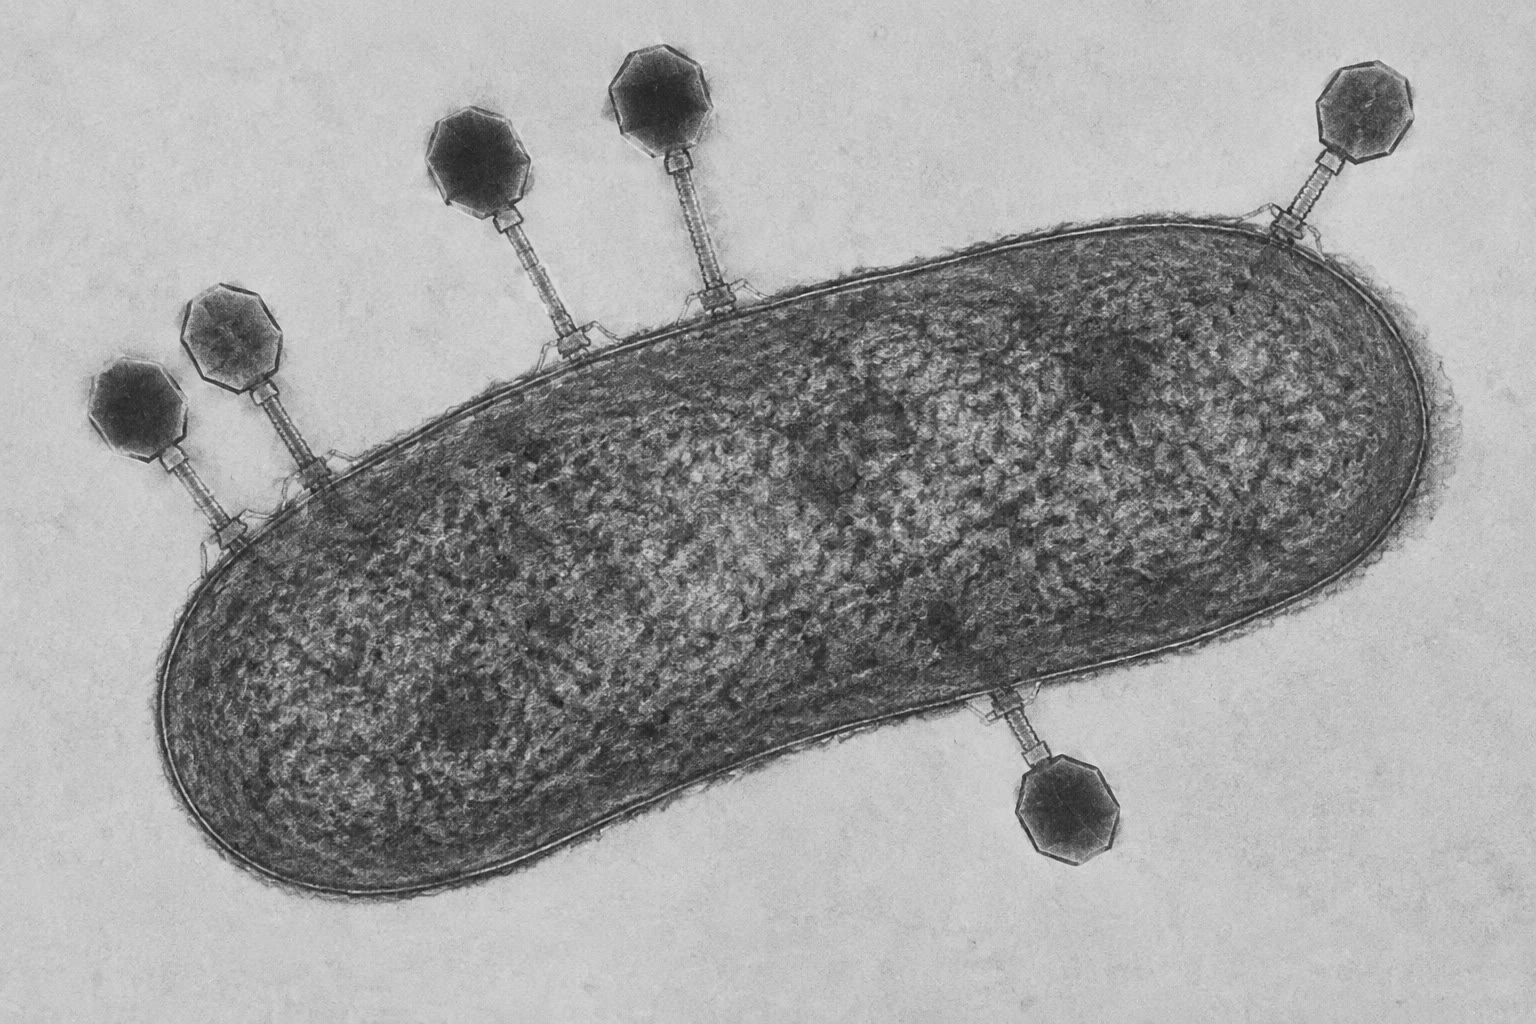
\includegraphics[width=0.5\linewidth]{images/book3/ai/b3-17-phage-on-bacterium.jpg}

{\small किसी जीवाणु से चिपके जीवाणुभोजी: बहुफलकी सिर, जिनमें \omterm{def:b1:nucleic-acids:chain}{DNA} है, और
पूँछें, जिनसे उसे भीतर डाला जाएगा। एक ही \omterm{def:b1:cell-unit-of-life:cell}{कोशिका} आधे घंटे के भीतर सौ नए
भोजी छोड़ देगी।}
\end{omfigure}

\begin{proposition}[फ़ेज $\lambda$ के दो चक्र]\label{prop:b1:genomes:lambda}
\index{लयन चक्र}\index{लयजनी चक्र}
फ़ेज $\lambda$ अपने \qty{48.5}{kb} \omterm{def:b1:nucleic-acids:chain}{DNA} (\cref{ch:b1:nucleic-acids}) को
\emph{E. coli} में डाल देता है, जहाँ वह वृत्ताकार हो जाता है। उसके बाद दो
नियतियाँ हैं। \emph{\omterm{prop:b1:genomes:lambda}{लयन चक्र}} में फ़ेज के \omterm{def:b1:genomes:gene}{जीन} पोषी के पॉलिमरेज़ से
अनुलेखित होते हैं, उसका \omterm{def:b1:nucleic-acids:chain}{DNA} सौ गुना प्रतिकृत होता है, \omterm{def:b1:genomes:virus}{कैप्सिड} \omterm{def:b1:proteins:peptide}{प्रोटीन}
बनते और जुड़ते हैं, \omterm{def:b1:nucleic-acids:chain}{DNA} उनमें भर दिया जाता है, और कोई \omterm{def:b1:enzymes:enzyme}{एंजाइम} भित्ति गला
देता है: संक्रमण के चालीस मिनट बाद \omterm{def:b1:cell-unit-of-life:cell}{कोशिका} फट जाती है और सौ फ़ेज छोड़ देती
है। \emph{\omterm{prop:b1:genomes:lambda}{लयजनी चक्र}} में फ़ेज का \omterm{def:b1:nucleic-acids:chain}{DNA} पोषी \omterm{def:b1:genomes:genome}{गुणसूत्र} में डाल दिया
जाता है और उसके अपने बनाए किसी दमनकारी से चुप करा दिया जाता है:
\emph{पूर्वफ़ेज} पीढ़ियों तक \omterm{def:b1:genomes:genome}{गुणसूत्र} के साथ नक़ल होता रहता है, अदृश्य,
जब तक पोषी के \omterm{def:b1:nucleic-acids:chain}{DNA} को हुई कोई क्षति उस दमन को हटा न दे और \omterm{prop:b1:genomes:lambda}{लयन चक्र} फिर
शुरू न हो जाए। यह चुनाव एक आणविक स्विच है, और सबसे पहले समझे गए स्विचों
में से एक (\cref{ch:b1:expression-control})।
\end{proposition}

\begin{omfigure}
\begin{tikzpicture}[font=\footnotesize, >=Stealth, line cap=round,
  st/.style={draw, thick, rounded corners=3pt, inner sep=3pt, align=center, fill=white}]
  \node[st, fill=omDef!12] (inj) at (0,0) {फ़ेज DNA भीतर डाला गया,\\ वृत्ताकार हुआ};
  \node[st, fill=omThm!12] (rep) at (4.6,1.4) {प्रतिकृतिकरण, कैप्सिड\\ प्रोटीन, संयोजन};
  \node[st, fill=omThm!12] (lys) at (9.2,1.4) {लयन: \qty{100}{} फ़ेज\\ छूटे, \qty{40}{min}};
  \node[st, fill=omExo!12] (pro) at (4.6,-1.4) {पूर्वफ़ेज के रूप में जुड़ा,\\ अपने दमनकारी से चुप};
  \node[st, fill=omExo!12] (div) at (9.2,-1.4) {पीढ़ियों तक पोषी गुणसूत्र\\ के साथ नक़ल होता};
  \draw[->, thick, omThm] (inj) -- (rep) node[pos=0.45, above left, omThm] {लयन};
  \draw[->, thick, omThm] (rep) -- (lys);
  \draw[->, thick, omExo!70!black] (inj) -- (pro) node[pos=0.4, below left, omExo!70!black] {लयजनी};
  \draw[->, thick, omExo!70!black] (pro) -- (div);
  \draw[->, thick, dashed, gray] (div.north) -- (lys.south) node[midway, right, align=left, font=\scriptsize] {प्रेरण\\ (पोषी DNA क्षतिग्रस्त)};
\end{tikzpicture}

{\small फ़ेज $\lambda$: \omterm{prop:b1:genomes:lambda}{लयन चक्र} (लाल) या लयजनी (हरा), और
वह प्रेरण जो दूसरे को पहला बना देता है।}
\end{omfigure}

\begin{example}[RNA जीनोम वाले विषाणु]\label{ex:b1:genomes:rna}
इन्फ़्लुएंज़ा एकलड़ी \omterm{def:b1:nucleic-acids:chain}{RNA} के आठ खंड ढोता है और उन्हें नक़ल करने के लिए
अपना ही पॉलिमरेज़, क्योंकि \omterm{def:b1:cell-unit-of-life:cell}{कोशिकाओं} में \omterm{def:b1:nucleic-acids:chain}{RNA} की नक़ल करने वाला कोई \omterm{def:b1:enzymes:enzyme}{एंजाइम}
नहीं होता; उसका पॉलिमरेज़ प्रति \num{10000} क्षारक एक भूल करता है और
\omterm{def:b1:genomes:virus}{विषाणु} हर ऋतु में बदल जाता है। कोई प्रतिवर्ती \omterm{def:b1:genomes:virus}{विषाणु} (HIV) \omterm{def:b1:nucleic-acids:chain}{RNA} और एक
\emph{प्रतीप अनुलेखेज़} ढोता है जो उसे \omterm{def:b1:nucleic-acids:chain}{DNA} में नक़ल कर देता है, और वह
पोषी \omterm{def:b1:genomes:genome}{गुणसूत्र} में किसी पूर्वफ़ेज की तरह डाल दिया जाता है --- यानी एक
स्थायी संक्रमण। क्रियाविधियाँ, और उनके प्रति प्रतिरक्षा अनुक्रिया, वर्ष 3
के खंड की हैं; यहाँ वे बस यह दिखाते हैं कि \omterm{def:b1:genomes:genome}{जीनोम} कितनी तरह का हो सकता है।
\end{example}

\section{अभ्यास}

\begin{exercise}[$\star$]\label{exo:b1:genomes:1}
जीवाणु और \omterm{def:b1:cell-unit-of-life:prokeuk}{सुकेंद्रकी} \omterm{def:b1:genomes:genome}{जीनोम} की तुलना कीजिए: \omterm{def:b1:genomes:genome}{गुणसूत्रों} की संख्या तथा
आकृति, स्थान, उन्हें सजाने वाले \omterm{def:b1:proteins:peptide}{प्रोटीन}, और जीन-घनत्व।
\end{exercise}

\begin{exercise}[$\star$]\label{exo:b1:genomes:2}
किसी \omterm{def:b1:genomes:nucleosome}{न्यूक्लियोसोम} का वर्णन कीजिए और \omterm{def:b1:genomes:nucleosome}{क्रोमैटिन} के मुड़ाव के हर स्तर का
संहतीकरण गुणक दीजिए।
\end{exercise}

\begin{exercise}[$\star$]\label{exo:b1:genomes:3}
जनगणना वाले आलेख से बताइए कि मानव \omterm{def:b1:genomes:genome}{जीनोम} का कितना भिन्न \omterm{def:b1:proteins:peptide}{प्रोटीन} के लिए कूट
करता है, और सबसे बड़ी श्रेणी कौन-सी है।
\end{exercise}

\begin{exercise}[$\star$]\label{exo:b1:genomes:4}
\omterm{def:b1:genomes:virus}{विषाणु} क्या है, और किस अर्थ में वह जीवित नहीं है?
\end{exercise}

\begin{exercise}[$\star\star$]\label{exo:b1:genomes:5}
\emph{E. coli} \omterm{def:b1:genomes:genome}{गुणसूत्र} की लंबाई निकालिए और वे न्यूक्लियोसोम-आकार के फेरे
भी जो उसे चाहिए होते यदि वह \omterm{def:b1:cell-unit-of-life:prokeuk}{सुकेंद्रकी} होता; और समझाइए कि जीवाणु उसे
इसकी जगह कैसे संहत करता है।
\end{exercise}

\begin{exercise}[$\star\star$]\label{exo:b1:genomes:6}
\qty{27}{kb} के किसी मानव \omterm{def:b1:genomes:gene}{जीन} में आठ टुकड़ों में \qty{1.5}{kb} \omterm{def:b1:genomes:gene}{एक्सॉन}
हैं। माध्य \omterm{def:b1:genomes:gene}{एक्सॉन} तथा \omterm{def:b1:genomes:gene}{इंट्रॉन} लंबाइयाँ और प्राथमिक अनुलेख का वह भिन्न
निकालिए जो फेंक दिया जाता है।
\end{exercise}

\begin{exercise}[$\star\star$]\label{exo:b1:genomes:7}
सारणी से \emph{E. coli}, खमीर, फल-मक्खी, मनुष्य और फेफड़ा-मछली के लिए
प्रति मेगाक्षारक \omterm{def:b1:genomes:gene}{जीन} निकालिए। प्रवृत्ति पर टिप्पणी कीजिए।
\end{exercise}

\begin{exercise}[$\star\star$]\label{exo:b1:genomes:8}
Alu तत्व \qty{300}{bp} का है और दस लाख प्रतियों में मौजूद।
\omterm{def:b1:genomes:genome}{जीनोम} का कितना भिन्न Alu है? यदि हर प्रति प्रतीप-स्थानांतरण से उठी हो
(यानी किसी \omterm{def:b1:nucleic-acids:chain}{RNA} की वापस \omterm{def:b1:nucleic-acids:chain}{DNA} में नक़ल और उसका प्रवेश), तो
\num{20} वर्ष प्रति पीढ़ी की दर से \num{60} लाख वर्षों में दस लाख
प्रतियाँ बनाने के लिए प्रति पीढ़ी कितने प्रवेश चाहिए होंगे?
\end{exercise}

\begin{exercise}[$\star\star$]\label{exo:b1:genomes:9}
समझाइए कि \omterm{def:b1:eukaryotic-cell:mitochondrion}{सूत्रकणिका} \omterm{def:b1:genomes:genome}{जीनोम} मातृ-वंशागत क्यों होता है, और वंशावली खोजने के
लिए इससे क्या निकलता है।
\end{exercise}

\begin{exercise}[$\star\star\star$]\label{exo:b1:genomes:10}
लयजनी अवस्था में फ़ेज $\lambda$ प्रति पोषी पीढ़ी एक बार नक़ल होता है;
लयन अवस्था में वह \qty{40}{min} में सौ प्रतियाँ बना लेता है।
हर \qty{20}{min} में दुगुने होते किसी भरपेट संवर्धन में दो घंटे तक दोनों
नीतियों की तुलना कीजिए; और ऐसे किसी भूखे संवर्धन में जो विभाजित नहीं
होता, फिर से तुलना कीजिए। यह स्विच पोषी की दशा के प्रति अनुक्रिया क्यों
करता है?
\end{exercise}

\begin{exercise}[$\star\star\star$]\label{exo:b1:genomes:11}
किसी फेफड़ा-मछली की \omterm{def:b1:cell-unit-of-life:cell}{कोशिका} \qty{130}{Gb} ढोती है: \omterm{def:b1:nucleic-acids:chain}{DNA} की लंबाई,
\omterm{def:b1:genomes:nucleosome}{न्यूक्लियोसोमों} की संख्या, प्रति \omterm{def:b1:cell-unit-of-life:cell}{कोशिका} \omterm{def:b1:genomes:nucleosome}{हिस्टोनों} का द्रव्यमान, और
प्रति \qty{100}{kb} एक उद्गम के साथ मानव द्विशाख-चाल (\qty{50}{bp/s} प्रति
द्विशाख) पर उसे प्रतिकृत करने का समय निकालिए। किसी बड़े \omterm{def:b1:genomes:genome}{जीनोम} की \omterm{def:b1:cell-unit-of-life:cell}{कोशिका}
को क्या क़ीमत चुकानी पड़ती है?
\end{exercise}

\begin{exercise}[$\star\star\star$]\label{exo:b1:genomes:12}
``\omterm{def:b1:genomes:genome}{जीनोम} एक अभिलेख है, कोई अभिकल्पना नहीं।'' छद्मजीनों, स्थानांतरणीय
तत्वों, \omterm{def:b1:genomes:gene}{जीन} कुलों और \omterm{prop:b1:genomes:cvalue}{C-मान विरोधाभास} की सहायता से एक अनुच्छेद में चर्चा
कीजिए।
\end{exercise}

\section{समस्या: छह माइक्रोमीटर में दो मीटर}

\begin{problem}[{सप्ताहांत समस्या --- कुंडली से गुणसूत्र तक मापा गया एक
मानव केंद्रक: हर स्तर पर लंबाइयाँ, आयतन, न्यूक्लियोसोम, हिस्टोन और
जमाव-अनुपात, और अंत में मध्यावस्था का कुल संहतीकरण}]
\label{pb:b1:genomes:1}
कोई मानव द्विगुणित केंद्रक \qty{6}{\micro m} व्यास का एक गोला है जो
46 \omterm{def:b1:genomes:genome}{गुणसूत्रों} पर $\num{6.4e9}$ \omterm{thm:b1:nucleic-acids:helix}{क्षारक युग्म} रखता है; सबसे बड़ा
\omterm{def:b1:genomes:genome}{गुणसूत्र} \qty{250}{Mb} ढोता है, सबसे छोटा \qty{50}{}।
प्रति युग्म \qty{0.34}{nm}, कुंडली का व्यास \qty{2}{nm},
प्रति युग्म \qty{650}{Da}, प्रति \omterm{def:b1:genomes:nucleosome}{न्यूक्लियोसोम} \num{200} युग्म, \omterm{def:b1:genomes:nucleosome}{हिस्टोन}
अष्टक \qty{108}{kDa}, और प्रति डाल्टन $\qty{1.66e-24}{g}$ लीजिए।

\medskip
\noindent\textbf{भाग I --- लंबाइयाँ और आयतन।}
\begin{enumerate}
  \item केंद्रक में \omterm{def:b1:nucleic-acids:chain}{DNA} की कुल लंबाई निकालिए।
  \item उसमें द्विकुंडली के फेरों की संख्या निकालिए।
  \item सबसे बड़े और सबसे छोटे \omterm{def:b1:genomes:genome}{गुणसूत्र} के \omterm{def:b1:nucleic-acids:chain}{DNA} की लंबाई निकालिए।
  \item केंद्रक का आयतन निकालिए।
  \item \omterm{def:b1:nucleic-acids:chain}{DNA} का आयतन किसी बेलन के रूप में निकालिए, और केंद्रक का वह
        भिन्न भी जो वह घेरता है।
  \item केंद्रक में \omterm{def:b1:nucleic-acids:chain}{DNA} का द्रव्यमान पिकोग्राम में निकालिए।
  \item केंद्रक में लगभग \qty{25}{pg} \omterm{def:b1:proteins:peptide}{प्रोटीन} है। यदि केंद्रक का
        \qty{80}{\%} जल हो (घनत्व \qty{1.1}{g/mL}), तो केंद्रकी
        द्रव्यमान का कितना भिन्न \omterm{def:b1:nucleic-acids:chain}{DNA} है?
\end{enumerate}

\medskip
\noindent\textbf{भाग II --- \omterm{def:b1:genomes:nucleosome}{न्यूक्लियोसोम}।}
\begin{enumerate}[resume]
  \item केंद्रक में \omterm{def:b1:genomes:nucleosome}{न्यूक्लियोसोमों} की संख्या निकालिए।
  \item \omterm{def:b1:genomes:nucleosome}{हिस्टोनों} का द्रव्यमान निकालिए और \omterm{def:b1:nucleic-acids:chain}{DNA} के द्रव्यमान से तुलना
        कीजिए।
  \item एक \omterm{def:b1:genomes:nucleosome}{न्यूक्लियोसोम} के \qty{200}{} युग्म कुंडली के \qty{68}{nm}
        घेरते हैं पर \qty{11}{nm} लंबे किसी मनके में समा जाते हैं।
        ``डोरी पर मनकों'' का संहतीकरण गुणक निकालिए।
  \item \qty{30}{nm} तंतु अपनी लंबाई के प्रति \qty{11}{nm} छह
        \omterm{def:b1:genomes:nucleosome}{न्यूक्लियोसोम} रखता है। नंगे \omterm{def:b1:nucleic-acids:chain}{DNA} के सापेक्ष उसका संहतीकरण गुणक
        निकालिए।
  \item पूरे \omterm{def:b1:genomes:genome}{जीनोम} के लिए \qty{30}{nm} तंतु की लंबाई निकालिए, और उसकी
        तुलना केंद्रक के व्यास से कीजिए।
  \item \omterm{def:b1:nucleic-acids:chain}{DNA} के प्रतिकृत या अनुलेखित होने पर हर \omterm{def:b1:genomes:nucleosome}{न्यूक्लियोसोम} को खोलकर
        फिर जोड़ना पड़ता है। S प्रावस्था (\qty{8}{h}) में कितने
        \omterm{def:b1:genomes:nucleosome}{न्यूक्लियोसोम} फिर जोड़े जाते हैं? प्रति सेकंड कितने?
\end{enumerate}

\medskip
\noindent\textbf{भाग III --- फंदे और \omterm{def:b1:genomes:genome}{गुणसूत्र}।}
\begin{enumerate}[resume]
  \item \qty{30}{nm} तंतु के \qty{75}{kb} के फंदे किसी ढाँचे से लटकते
        हैं। एक फंदे में तंतु की लंबाई और \omterm{def:b1:genomes:genome}{जीनोम} में फंदों की संख्या
        निकालिए।
  \item सबसे बड़े \omterm{def:b1:genomes:genome}{गुणसूत्र} की कोई मध्यावस्था क्रोमैटिड
        \qty{10}{\micro m} लंबी है। नंगे \omterm{def:b1:nucleic-acids:chain}{DNA} से मध्यावस्था \omterm{def:b1:genomes:genome}{गुणसूत्र} तक
        संहतीकरण गुणक निकालिए।
  \item उस क्रोमैटिड का आयतन \qty{0.7}{\micro m} व्यास के किसी बेलन के
        रूप में निकालिए, और उसका वह भिन्न भी जो \omterm{def:b1:nucleic-acids:chain}{DNA} है।
  \item मध्यावस्था के 46 \omterm{def:b1:genomes:genome}{गुणसूत्र}, जिनमें से हर एक उसी घनत्व की छड़ है:
        उनका कुल आयतन निकालिए और अंतरावस्था के केंद्रक से तुलना कीजिए।
  \item समझाइए कि अंतरावस्था की \omterm{def:b1:genomes:nucleosome}{क्रोमैटिन} मध्यावस्था की \omterm{def:b1:genomes:nucleosome}{क्रोमैटिन} जितनी
        कसकर क्यों नहीं जमाई जा सकती।
\end{enumerate}

\medskip
\noindent\textbf{भाग IV --- कोई \omterm{def:b1:genomes:gene}{जीन} ढूँढ़ना।}
\begin{enumerate}[resume]
  \item किसी \omterm{def:b1:proteins:peptide}{प्रोटीन} को \omterm{def:b1:genomes:genome}{जीनोम} में \qty{20}{bp} का एक स्थल ढूँढ़ना है।
        यदि वह प्रति मिलीसेकंड एक यादृच्छिक स्थल जाँचे तो खोज में कितना
        समय लगता? इससे इस बारे में क्या पता चलता है कि स्थल कैसे ढूँढ़े
        जाते हैं?
  \item \omterm{def:b1:genomes:genome}{जीनोम} के \qty{20000}{} \omterm{def:b1:genomes:gene}{जीनों} का औसत \qty{27}{kb} है। \omterm{def:b1:genomes:genome}{जीनोम} का
        कितना भिन्न \omterm{def:b1:genomes:gene}{जीनों} के भीतर है? और प्रति \omterm{def:b1:genomes:gene}{जीन} \qty{1.5}{kb}
        \omterm{def:b1:genomes:gene}{एक्सॉन} पर कितना भिन्न कूटलेखी है?
  \item हर \omterm{def:b1:genomes:genome}{गुणसूत्र} केंद्रक में अपना ही क्षेत्र घेरता है।
        यदि क्षेत्र \omterm{def:b1:nucleic-acids:chain}{DNA} की मात्रा के समानुपाती हों, तो सबसे बड़े
        \omterm{def:b1:genomes:genome}{गुणसूत्र} के क्षेत्र का आयतन निकालिए, और उसके भीतर \omterm{def:b1:nucleic-acids:chain}{DNA} की
        सांद्रता \omterm{thm:b1:nucleic-acids:helix}{क्षारक युग्म} प्रति घन माइक्रोमीटर में भी।
  \item उसी \omterm{def:b1:nucleic-acids:chain}{DNA} घनत्व वाले किसी फेफड़ा-मछली के केंद्रक का
        \qty{260}{Gb} (द्विगुणित) के लिए आयतन क्या होगा? व्यास क्या?
  \item S प्रावस्था में \omterm{def:b1:cell-unit-of-life:cell}{कोशिका} को कितने \omterm{def:b1:genomes:nucleosome}{हिस्टोन} अष्टक बनाने पड़ते हैं
        और उनमें कितने \omterm{def:b1:proteins:aminoacid}{ऐमीनो अम्ल} हैं (प्रति अष्टक \qty{1000}{}
        अवशेष), यह निकालिए। \omterm{def:b1:cell-unit-of-life:cell}{कोशिका} एक दिन में जो \qty{3e9}{} \omterm{def:b1:proteins:peptide}{प्रोटीन}
        अवशेष बनाती है उनसे तुलना कीजिए।
  \item दो वाक्यों में समझाइए कि जीवाणु \omterm{def:b1:genomes:nucleosome}{न्यूक्लियोसोमों} के बिना काम क्यों
        चला लेते हैं और \omterm{def:b1:cell-unit-of-life:prokeuk}{सुकेंद्रकी} क्यों नहीं।
  \item परिणाम बताइए: कुंडली से मध्यावस्था \omterm{def:b1:genomes:genome}{गुणसूत्र} तक कुल संहतीकरण
        गुणक, और हर स्तर के गुणक।
\end{enumerate}
\end{problem}
